% #########################################################################
% #                       EXPLORACIÓN Y ANÁLISIS DE DATOS                 #
% #########################################################################

% Definición de nombres
\newcommand{\estudiante}{García Justel, Alan}
\newcommand{\titulo}{MÁSTER EN INGENIERÍA COMPUTACIONAL Y SISTEMAS INTELIGENTES}
\newcommand{\asignatura}{INTRODUCTION TO TIME SERIES DATA}
\newcommand{\portada}{common/no_signal.png}
\newcommand{\colorportada}{title_green}
\newcommand{\curso}{2024-2025}


% Notebook
\begin{document}
\newgeometry{bottom=2cm}

\begin{titlepage}
    % Logo de la universidad
    \begin{textblock*}{\textwidth}(2cm,0.4cm)
        \begin{center}
            \begin{minipage}{0.45\textwidth}
                \centering
                
\includegraphics[width=\textwidth]{common/Logo_EHU.jpg}
            \end{minipage}\hfill
            \begin{minipage}{0.45\textwidth}
                \centering
                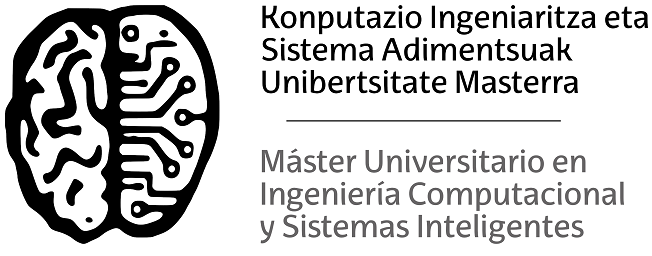
\includegraphics[width=0.8\textwidth]{common/Logo_KISA.png} 
            \end{minipage}
        \end{center}
    \end{textblock*}
    
    % Franja de color
    \begin{tikzpicture}[remember picture, overlay]
        \fill[\colorportada] (current page.north west) ++ (0,-3.01cm) rectangle (\paperwidth,-3cm);
    \end{tikzpicture}
    
    \begin{textblock*}{\paperwidth}(\dimexpr\parindent+\oddsidemargin+3em\relax,3.5cm)
        \begin{minipage}{\dimexpr\linewidth-7.5cm\relax}
            \color{white}
            \noindent\rule{\linewidth}{0cm}
            \textsf{ {\large \titulo}}
            \newline
            \newline \newline
            \textsf{\textbf{ {\Huge APUNTES DE ASIGNATURA }}}
        \end{minipage}
    \end{textblock*}
    
    % Nombre asignatura
    \vspace*{3.5cm}
    \begin{minipage}{\linewidth}
        \setlength{\baselineskip}{1.7\baselineskip}
        \centering
        \textsf{ \textbf{ {\LARGE \asignatura }}}
    \end{minipage}

    % Foto de portada
    \vspace*{0.5cm}
    \begin{figure}[H]
        \centering
        \includegraphics[width=10cm, height=8cm]{\portada}
    \end{figure}

    
    
    % Estudiante
    \vspace{0.2cm}
    \noindent {\footnotesize \textbf{Estudiante:} \estudiante}
    \newline
    \noindent\makebox[\linewidth]{\rule{\textwidth}{0.4pt}} % Línea horizontal

    % Curso y Fecha
    \vspace{0.1cm}    
    \noindent {\footnotesize \textbf{Curso: } \curso \hfill \textbf{Fecha:} \today }
\end{titlepage}

\restoregeometry
\setcounter{figure}{0} % Incluimos el título
\newpage
% Índices
\tableofcontents\thispagestyle{empty} \newpage
% \listoffigures\thispagestyle{empty}   %\newpage
% \listoftables\thispagestyle{empty}    %\newpage

\section{Introduction}
Time series data is information that represents one or more attributes (variables) over time (or another ordered dimension).
There are multiple aproximation for using a time series data for different tasks:
- Use the data directly or with a preprocessing step for noise and dimensionality reduction, split into windows of data, selecting specific parameter for represanting the time series data or other more sophisticated techniques like fourier methods.
- Use algorithms for specific data (convolutional networks for images, RNN for audio...).

\section{Time Series Forecasting}
The objective is to predict or to infer a future timestamp state for the time series.

$$
y_{t + a} = f(y_t, y_{t-1}, y_{t-2}, y_{t-3}, \dots, \text{error})
$$

Where $(y_{t}, y_{t}, y_{t})$ are the previous observations of the variables we want to predict (historical values). 
Also, it is possible to have other extra information ($(x_{1}, x_{2}, x_{3})$) that is useful for the forecasting:

$$
y_{t + a} = f(y_t, y_{t-1}, y_{t-2}, y_{t-3}, \dots, x_{1}, x_{2}, x_{3}, \dots, \text{error})
$$

\subsection{Classical lineal models}
The Classical lineal models has these assumptions:

\begin{itemize}
    \item \textbf{stochastic process}: an ordered sequence of random variables, where the
    order is typically given by time: $(Y_1, Y_2, Y_3, \dots, Y_n, \dots)$.
    \item \textbf{Time series}: a finite set of observations (a sample) from a real-valued
    stochastic process (univariate or multivariate).
\end{itemize}

We need a time series to be stationary in order to apply forecasting methods. A time series is stationary if these conditions are fulfilled:
$$
F(X_1, X_2, X_3, \dots, X_n) = P(X_1 < x_1, X_2 < x_2, X_3 < x_3, \dots, X_n < x_n)
$$
\begin{enumerate}
    \item First order stationary: $F(X_t) = F(X_{t +k})$. If the probability distribution of the first variable is the same as the second one, the same as the third one and so on.
    \item Second order stationary: $F(X_{t1}, X_{t2}) = F(X_{t1 + k}, X_{t2 + k})$.
\end{enumerate}

However, it is very difficult to have a full stationary time series, so a \textit{weak stationary} is defined:
\begin{enumerate}
    \item The mean is constant. $E(X_t)$
    \item The variance is constatnt. $\text{Var}(X_t)$
    \item The covariance si constant in terms of a parameter ($\text{Cov}(X_i, X_{i+k})=f(k)$). It depends on time difference between the random variables.
\end{enumerate}

\textbf{How do we check if a time series is stationary?}
\begin{enumerate}
    \item Visual inspection
    \item Statistical tests
\end{enumerate}

\textbf{Forecasting models for stationary time series:}
\begin{itemize}
    \item Autoregresive Models AR($p$): \textit{predict the future based on previous observations.} $X_t = f(X_{t-1}, \dots, X_{t_-p}) + \epsilon_t$
    \item Moving Average Models MA($q$): \textit{predict the future based on previous errors.} $X_t = f(\epsilon_{t-1}, \dots, \epsilon_{t_-q}) + \epsilon_t$
    \item ARMA Models: \textit{linear regression of previous observations and previous errors}.
\end{itemize}
AR, MA and ARMA processes will only fit if the original time series is stationary. There is a variation named ARIMA Models wich tries to fit an ARMA model but performing differenciation on the time series previously in order to make a non-stationary time series stationary. It has 3 parameters: $p$, from the AR part; $d$, from the differenciation part and $q$, from the MA part. There are also other extensions and variants such as ARIMAX... \textit{Auto-ARIMA} is an implementation of the ARIMA algorithm with some heuristics to search for the optimal hiperparámeters of the ARIMA model.

\textbf{Evaluation of a time series model:}

Evaluate if the residuals are white noise or not. Evaluate the prediction power of the model with metrics such as:
$$
RMSE = \sqrt{\frac{\sum_{t=1}^{N}(x_t - \hat{x}_t)^2}{N}}
$$

For cross validation see \href{https://topepo.github.io/caret/data-splitting.html}{Data splitting for Time Series}.


\section{Distances for Time Series}
There are two mainly aproximations for measuring the distance or similarity between two time series: fixed and flexible distances.

\textbf{Euclidean distance:} It is very simple to use and it hsa a low computational cost. However, it can only be used to compare series of the same lenght, the temporal correlation is not taken into account and it is very susceptible to noise.

\textbf{Dynamic Time Warping:} It takes the temporality into account and can be used to compare series of different lenghts.However, it is not a metric (does not fullfil triangle inequality) and it has a high computational cost: 
$$
    O(m*n) \text{ where } m,n =\text{lenghts of the time series}
$$ 

\textbf{Edit Distances:} One approach may be to calculate a binary distances matrix between the $m$ and $n$ time series using $d(x_i, y_i) < \epsilon$ for then applying the \textit{Dynamic Time Warping} algorithm. This method has some advantajes compared with the \textit{Dynamic Time Warping} such as it may be more robust to noise spikes.


\section{Time Series Classification}

\subsection{Feature based classification}
Represent the timeseries using a set of features. The representation doesn't depend on the number of training series and it is interpretable. However, there are some challenges such as what features do we have to select.

\subsection{Model based classification}
Train a distinct model for each class and when a new instance comes select the class of the model that gives the lowest error. It works well with models that fits the data, but it is very difficult to achieve this.

\subsection{Distance based classification}
These are currently the most popular methods for time series classification. 

\subsubsection{K-NN}
The most direct, simple and that achives good results stablishing a baseline for time series classification is $\text{K-NN} + \text{DTW}$ (usually with $K=1$). However, it is computational expensive and it is difficult to choose a distance method.

\subsubsection{Distance features}
\textbf{Distance based global classification} is a technique where any standar classifier is trained with the distances between all the training time series and new instances are classified using it's distances to all the training data.

\textbf{Distance based local features} are based on \textit{shapelets}, or small parts of the time series that has some identifying patterns used too differenciate between the classes. Once the \textit{shapelets} have been identified, any classical classifier can be trained with the distance matrix between the time series to the \textit{shapelets}. This method is very very very computational expensive. However, if \textit{shapelets} are relevant, this methods gives very good interpretable results.

\textbf{Embeded features} ...

\subsubsection{Distance Kernels}
The objective is to include kernel similarities in \textit{DTW} methods in order to apply algorithms shuch as \textit{SVMs} or \textit{GPs}. However, as DTW is not a metric, there are two main aproximations for this problem: to use specific matematical kernels or to tune the distances matrix in order to fullfil the metric conditions (semi-positive defined matrix).

\end{document}